\documentclass[a4paper]{article}
\usepackage[utf8]{inputenc}
\usepackage{fontspec}
\setsansfont{CMU Sans Serif}
\setmainfont{CMU Serif}
\setmonofont{CMU Typewriter Text}

\usepackage{graphicx}
\usepackage{booktabs}
\usepackage{xcolor}
\usepackage{listings}
\usepackage{microtype}
\usepackage{syntax}
\usepackage{amsmath}
\usepackage[super]{nth}
\usepackage{tikz}
\usepackage{tikz-qtree}
\usetikzlibrary{shapes,patterns,positioning,trees}
\usepackage[
  colorlinks,
  linkcolor={red!40!black},
  citecolor={blue!60!black},
  urlcolor={blue!60!black}
]{hyperref}
\usepackage{glossaries-extra}

\title{Filesystems}
\author{Patrick M. Elsen <pelsen@xfbs.net>}
\date{\today}

\setabbreviationstyle{long-short-sc}
\newabbreviation{fat}{fat}{File Allocation Table}
\newabbreviation{ext}{ext}{Extended File System}
\newabbreviation{ntfs}{ntfs}{New Technology File System}
\newabbreviation{uid}{uid}{User ID}
\newabbreviation{gid}{gid}{Group ID}
\newabbreviation{fifo}{fifo}{First In, First Out}
\newabbreviation{ipc}{ipc}{Interprocess Communication}
\newabbreviation{icmp}{icmp}{Internet Control Message Protocol}
\newabbreviation{acl}{acl}{Access Control Lists}
\newabbreviation{posix}{posix}{Portable Operating Systems Interface}
\newabbreviation{gui}{gui}{Guided User Interface}
\newabbreviation{sip}{sip}{System Integrity Protection}
\newabbreviation{api}{api}{Application Programming Interface}
\newabbreviation{hfs+}{hfs+}{Hiearchical File System Plus}
\newabbreviation{apfs}{apfs}{Apple File System}
\newabbreviation{ssd}{ssd}{Solid State Drive}
\makeglossaries

% don't show subsubsections in toc
\addtocontents{toc}{\setcounter{tocdepth}{2}}

\begin{document}

\maketitle

\tableofcontents

\section{Introduction}

Filesystems have always been fascinating to me. They are a kind of ubiquitous database. A lot of work goes into developing and making them work. And yet, a lot of information about them is relatively unknown. In this article, I set forth to explore some of their features.

We will look at what kinds of filesystems exist in the Linux kernel, and how they differ. We will look at the API that is presented to the user. We will also explore some advanced filesystem features and even implement our own little FS with FUSE.

All that is required for following along is a bit of experience with the Linux command line. MacOS also works, but has a slightly different set of features that are also addressed. Windows users may want to install WSL, but we will also take a look at some Windows-specific quirks.

This document comes with some code for utilities to work with the file system. These should be compiled and used. All command line examples in this document use these utilities rather than similarly named ones shipped with your system, unless noted otherwise.

\section{History}

UNIX as an operating system took the concept of a file system and really took it to the next level. The idea was that \emph{everything} could be a file. We see this today by some of the well-known character devices such as \verb|/dev/null| or \verb|/dev/urandom|, which we can accesses using the filesystem metaphor, but aren't files on disk in the typical sense.

DOS, the predecessor of the popular Windows operating system, had a comparatively limited concept of a file system. Initially, it did not support hierarchies, meaning that there were no folders, and file names were limited to just 11 characters. As personal computers became more powerful, this put DOS at a disadvantage, which resulted in them fixing it, but it still leaves some cruft in the Windows world. For example, Windows has no folder like UNIX’es \verb|/dev|, but device files are present in any directory.

\section{Filesystems}

Filesystems define how the structures we can work with (directories, files) and their metadata are stored on disk. As such, they are implemented in the kernel. 

Finding out what filesystem is in use can be accomplished with the \emph{stat} command.

\begin{verbatim}
$ stat -f /
  File: "/"
    ID: a34c153af3f0097e Namelen: 255     Type: ext2/ext3
Block size: 4096       Fundamental block size: 4096
Blocks: Total: 40605120   Free: 35164744   Available: 35160648
Inodes: Total: 20643840   Free: 20461918
\end{verbatim}

In this case, we learn that the filesystem in use is from the \textsc{ext} family of filesystems, with a 4K block size.

The most common filesystem used on Linux is \verb|ext4|, but there are plenty others. Filesystems supported by Linux are \verb|ext|, \verb|ext2|, \verb|ext3|, \verb|ext4|, \verb|hpfs|, \verb|iso9660|, \verb|JFS|, \verb|minix|, \verb|msdos|, \verb|ncpfs nfs|, \verb|ntfs|, \verb|proc|, \verb|Reiserfs|, \verb|smb|, \verb|sysv|, \verb|umsdos|, \verb|vfat|, \verb|XFS|, \verb|xiafs|.

\subsection{\glsdesc*{ext} family}

The \gls{ext} family of filesystems derive from the \verb|minix| filesystem, that has been extensively extended to support additional metadata, journaling, and improve performance and reliability. Since this family of filesystems is very common on Linux machines, its feature set will be studied in-depth.

\subsection{\glsdesc*{fat} family}

The \verb|msdos|, \verb|umsdos| and \verb|vfat| filesystems all belong to the \gls{fat} family of filesystems designed by Microsoft in 1977. They have a lot of limitations compared to modern filesystems, but are very simple to implement, and hence \gls{fat} is still used today, for example required by the SD Consortium.

The principal difference between these drivers is the amount of emulation for \textsc{unix} features they provide. The \emph{msdos} driver supports almost no \textsc{unix} features, such as file permissions, attributes, and only filenames with a length of 8 characters, optionally followed by a dot and a three-character extension.

\subsection{\glsdesc*{ntfs}}

The \gls{ntfs} is the filesystem currently used by Windows. It supports a lot of the advanced features that modern filesystems have, and even some obscure ones like \emph{alternate file streams}.

\subsection{\glsdesc*{hfs+}}

The \gls{hfs+} is a filesystem currently used by Apple on their whole product range.

\subsection{\glsdesc*{apfs}}

The \gls{apfs} is a new filesystem developed by Apple and used across their product range. It is optimised for newer \gls{ssd} storage and has some unique features, such as filesystem snapshots, native full disk encryption, metadata integrity with checksums, and space sharing.

\section{File Hierachy}

In the \textsc{unix} world, the filesystem starts at the path \verb|/|. This is also called the \emph{root}. In this root, a number of directories typically exist, such as \verb|usr|, \verb|dev|, \verb|var|, \verb|bin|, and so forth.

\begin{verbatim}
$ ls /
bin  etc  lib64  mnt  run  tmp  boot   home 
lib  opt  root   src  usr  dev  lib32  media 
proc sbin sys   var
\end{verbatim}

Every entry in the file hiearchy has an \emph{inode} number associated with it, uniquely identifying the file (entry).

\subsection{File Hiearchy Standard}

\section{Entries}

A filesystem contains \emph{entries}. Every entry has a unique \emph{inode} associated with it. There are different kinds of entries. The most well-known entry types are \emph{regular files} and \emph{directories}. 

Using the \emph{stat} syscall, we can ask the kernel about information on an entry. The \emph{stat} bash command performs this syscall for us and returns the information in a readable way, including the type of an entry\footnote{For more information on this sycall, check \texttt{man 7 inode} and \texttt{man 2 stat}.}.

\begin{verbatim}
$ stat ~/.bashrc
  File: /home/patrick/.bashrc
  Size: 3771            Blocks: 8          IO Block: 4096   regular file
Device: fc01h/64513d    Inode: 258084      Links: 1
Access: (0644/-rw-r--r--)  Uid: ( 1000/ patrick)   Gid: ( 1000/ patrick)
Access: 2019-09-26 12:47:34.337622163 +0000
Modify: 2019-07-23 15:41:13.075202952 +0000
Change: 2019-07-23 15:41:13.075202952 +0000
 Birth: -  
\end{verbatim}
From this, we learn that \verb|~/.bashrc| is indeed a regular file. It is owned by the user with the \textsc{uid} 1000, which happens to be \emph{patrick}. 

\subsection{Directory}

A directory contains other entries. It can be created with \verb|mkdir| command. An empty directory can be deleted with \verb|rmdir|. Contents of a directory can be listed with the \verb|ls| command.

\begin{verbatim}
$ mkdir folder
$ rmdir folder  
\end{verbatim}
If a directory is not empty, it cannot be deleted with \verb|rmdir|.

\begin{verbatim}
$ mkdir folder
$ touch folder/file
$ rmdir folder
rmdir: failed to remove 'folder/': Directory not empty
\end{verbatim}
The \emph{stat} tool output of folders shows us that folders have the same metadata attached to them that regular files have.

\begin{verbatim}
  File: folder
  Size: 4096            Blocks: 8          IO Block: 4096   directory
Device: fc01h/64513d    Inode: 5680241     Links: 2
Access: (0775/drwxrwxr-x)  Uid: ( 1000/ patrick)   Gid: ( 1000/ patrick)
Access: 2019-09-26 13:49:04.481613173 +0000
Modify: 2019-09-26 13:49:09.853614507 +0000
Change: 2019-09-26 13:49:09.853614507 +0000
 Birth: -  
\end{verbatim}

The syscalls used to create, read and delete directories are \verb|mkdir()|, \verb|opendir()|, \verb|readdir()|, \verb|rewinddir()|, \verb|seekdir()|, \verb|telldir()|, \verb|scandir()|.

\subsection{Regular File}

Regular files are what we think of when we think of files. They contain data, and can be written to and read from.

\begin{verbatim}
$ echo hi > filename
$ cat filename
hi  
\end{verbatim}
The \emph{stat} tool output shows us that folders have a basic amount of metadata attached to them.

\begin{verbatim}
  File: file
  Size: 0               Blocks: 0          IO Block: 4096   regular empty file
Device: fc01h/64513d    Inode: 258817      Links: 1
Access: (0664/-rw-rw-r--)  Uid: ( 1000/ patrick)   Gid: ( 1000/ patrick)
Access: 2019-09-26 14:41:37.221013724 +0000
Modify: 2019-09-26 14:41:37.221013724 +0000
Change: 2019-09-26 14:41:37.221013724 +0000
 Birth: -
\end{verbatim}

Files can be created with the \verb|open()| sycall with the \verb|O_CREAT| flag, written and read to with \verb|write()| and \verb|read()|, and deleted with \verb|unlink()|.

\subsection{Symbolic Link}

Symbolic links are essentially files containing paths to the real file. When opening them, they act as a proxy to the real file. 

Syscalls used for creating and reading symbolic links are \verb|symlink()| and \verb|readlink()|.

\subsection{FIFO Queue}

\gls{fifo} queues are a type of special entry provided by the kernel. Unlike regular files, they don't store anything on disk. Rather, they are meant to be used by two processes, one process reading from it and the other writing to it. The data that is written is sent directly between these processes without being sent to disk first. Therefore, \gls{fifo} queues are a kind of \gls{ipc} mechanism.

\subsection{Socket}

Also called \textsc{unix} domain sockets, these are similar to network sockets in that they allow binding (listening for connections) and connecting, but without involving the network stack.

\subsection{Character Special File}

Character special files are entries that are handled completely by the kernel. They are identified by a pair of numbers, the minor and major number. Examples of this are \verb|/dev/null| and \verb|/dev/urandom|.

When reading or writing from them, the action that happens depends on their minor and major numbers in the kernel.

\subsection{Block Device}

\section{Permissions}

UNIX sports a very simple permissions model that is based on a bitmask. Every file has an owner (user) and a group associated with it. The permissions that can be given are \emph{read}, \emph{write} and \emph{execute} for each of the owner, the group and the world (anyone). In addition to that, there is a set of special flags that can be set on entries, which are \emph{set-user-\textsc{id}}, \emph{set-group-\textsc{id}} and the \emph{sticky bit}.

These permissions are typically either shown in octal form (such as 0755) or in text form.

\begin{table}[!h]
\centering\caption{List of Permissions}
\begin{tabular}{@{}lll@{}}
\toprule
\textbf{Name} & \textbf{Octal} & \textbf{String}\\
\midrule
Set user ID      & 4000 & \verb|---s------|\\
Set group ID     & 2000 & \verb|------s---|\\
Sticky bit       & 1000 & \verb|---------t|\\
Read by owner    & 0400 & \verb|-r--------|\\
Write by owner   & 0200 & \verb|--w-------|\\
Execute by owner & 0100 & \verb|---x------|\\
Read by group    & 0040 & \verb|----r-----|\\
Write by group   & 0020 & \verb|-----w----|\\
Execute by group & 0010 & \verb|------x---|\\
Read by world    & 0004 & \verb|-------r--|\\
Write by world   & 0002 & \verb|--------w-|\\
Execute by world & 0001 & \verb|---------x|\\
\bottomrule  
\end{tabular}
\end{table}
Permissions can be changed for files using the \emph{chmod} utility. An example of setting full read, write and execute permissions for owner, group and world might look like such.

\begin{verbatim}
$ touch file
$ chmod 0777 file
$ ls -l file
-rwxrwxrwx 1 patrick patrick 0 Sep 26 14:25 file  
\end{verbatim}
When removing read permissions, even the owner is unable to read from it.

\begin{verbatim}
$ touch file
$ chmod 0000 file
$ cat file
cat: file: Permission denied
\end{verbatim}

\subsection{Read}

\subsection{Write}

\subsection{Execute}

The execute bit has a different meaning for directories. If it is not set, the contents of the directory can't be enumerated with \verb|readdir()|. 

\subsection{Set UID and Set GID}

The \verb|setuid| bit are special in the sense that they change the effective \gls{uid} and \gls{gid} of the running process. Normally, when running an executable, the \gls{uid} and \gls{gid} are set to that of the user that executes it.

\begin{verbatim}
$ ./perms
uid 1000 (patrick)
gid 1000 (patrick)
euid 1000 (patrick)
egid 1000 (patrick)  
\end{verbatim}
However, when the Set \gls{uid} bit is set, then the effective \gls{uid} is set to that of the user who \emph{owns} the executable, rather than the one who runs it.

\begin{verbatim}
$ chown root perms
$ chmod u+s perms
$ ./perms
uid 1000 (patrick)
gid 1000 (patrick)
euid 0 (root)
egid 1000 (patrick)  
\end{verbatim}
This functionality is used in executables that need extra capabilities but should be usable by non-root users as well. Examples for this are the \verb|/bin/ping| utility, which needs raw access to generate \gls{icmp} ping packets, or \verb|/usr/bin/sudo|, which grants superuser rights to regular users depending on its configuration.

\subsection{Sticky bit}

The sticky bit has an effect on directories only. When set, files in the directory can be deleted or renamed only by the owner of the file, or the owner of the directory. This is used for directories like \verb|/tmp|, where anyone should be able to write into, but files should not be able to be deleted by anyone other than the user that created them.

\section{Quotas}

\subsection{User}

\subsection{Group}

\subsection{Project}

% https://lwn.net/Articles/623835/
% http://man7.org/linux/man-pages/man8/setquota.8.html

\section{Attributes}

Attributes are flags that can be set on filesystem entries. These attributes are, from what I can tell, not standardised across operating systems. 

\subsection{Linux}

Linux sports a number of attributes.

% man chattr
% man ioctl_iflags

\subsubsection{Append-only file}

The xxx.

\subsection{MacOS}

% help: what is https://ss64.com/osx/setfile.html setfile? 
% what does it do and how does it work?

% how are these flags different from attrs like getattrlist
% and setattrlist?

MacOS also supports file attributes, called \emph{flags}. They are returned in the \verb|sv_flags| field of the \verb|stat()| syscall. The \verb|stat| utility included in this project displays the flags set for a given file.

\begin{verbatim}
$ stat /bin | grep flags
flags: restricted,hidden
\end{verbatim}
Table \ref{tbl:macosflags} lists all flags currently known to and implemented in the MacOS kernel, as of the time of writing\footnote{\texttt{/Library/Developer/CommandLineTools/SDKs/MacOSX.sdk/usr/include/sys/stat.h} documents the currently known and used flags.}. Some flags are limited in that they can only be set by the superuser. 
\begin{table}
\centering\caption{MacOS File Attributes}\label{tbl:macosflags}
\begin{tabular}{@{}lp{10.5cm}@{}}
\toprule
Name & Description\\
\midrule
\emph{nodump} & Don't dump this file.\\
\emph{uchg} & File may not be changed.\\
\emph{uappnd} & File may only be appended to.\\
\emph{opaque} & Directory is opaque when viewed through a union mount.\\
\emph{hidden} & File or directory is hidden in the \gls{gui}.\\
\emph{arch} & File has been archived.\\
\emph{schg} & File may not be changed, even by the superuser.\\
\emph{sappnd} & File may only appended to, even by the superuser.\\
\emph{restricted} & File is under \gls{sip}.\\
\emph{nounlink} & File may not be removed, renamed or mounted on.\\
\bottomrule  
\end{tabular}
\end{table}

Apple's \gls{sip} uses the \emph{restricted} flag to mark files and folders as system folders, which cannot be set or unset by anyone unless \gls{sip} is turned off.

It is possible, on macOS, to view the file attributes using \verb|ls| with the \verb|O| flag. 

\begin{verbatim}
$ ls -oOd /bin /Volumes /net /private
drwxr-xr-x+  4 root  hidden             128 Sep 25 20:11 /Volumes
drwxr-xr-x@ 37 root  restricted,hidden 1184 Jun 12 15:54 /bin
dr-xr-xr-x   2 root  hidden               1 Sep 24 09:31 /net
drwxr-xr-x   6 root  sunlnk,hidden      192 Sep 27  2018 /private  
\end{verbatim}

% https://en.wikipedia.org/wiki/File_attribute

\subsubsection{Nodump}

The \emph{nodump} flag can be set by any regular user and signals to the \emph{dump} utility, which was used for backups in old versions of \textsc{unix} and is long obsolete, that this file should not be included in the dump.

\subsubsection{Uchg}

The \emph{uchg} flag signals to the kernel that this file is immutable and should not be able to be changed. It can be set by a regular user. It affects any user and prevents them from writing to, deleting or renaming the file until the flag is cleared.

\begin{verbatim}
$ flags file uchg
$ echo hi > file
-bash: file: Operation not permitted
$ echo hi | sudo tee file
tee: file: Operation not permitted
$ unlink file
file: Operation not permitted
$ flags file nouchg
$ unlink file
\end{verbatim}

\subsubsection{Uappnd}

The user append flag prevents a file from being overwritten, by only letting processes open it in append mode. It also prevents the file from being deleted with \verb|unlink()|, renamed or hard links to it being created. This flag can be set and unset by the owner of the file.

\begin{verbatim}
$ touch file
$ flags file uappnd
$ echo hi > file
-bash: file: Operation not permitted
$ echo hi >> file
\end{verbatim}

\subsubsection{Opaque}

The opaque flag plays a role when using a union mount. This happens when mounting a filesystem over another filesystem such that both are visible. When setting the opaque flag on a directory, then this union property does not work for the directory.

\subsubsection{Hidden}

The hidden flag hides files or folders that it is defined on from the GUI. 

\begin{verbatim}
$ ls
Makefile  fsdoc.tex src
$ flags Makefile hidden
$ open .
\end{verbatim}

See Figure \ref{fig:macoshidden} to see that the Makefile is indeed hidden from Finder.

\begin{figure}
\centering\caption{Hidden Makefile}\label{fig:macoshidden}
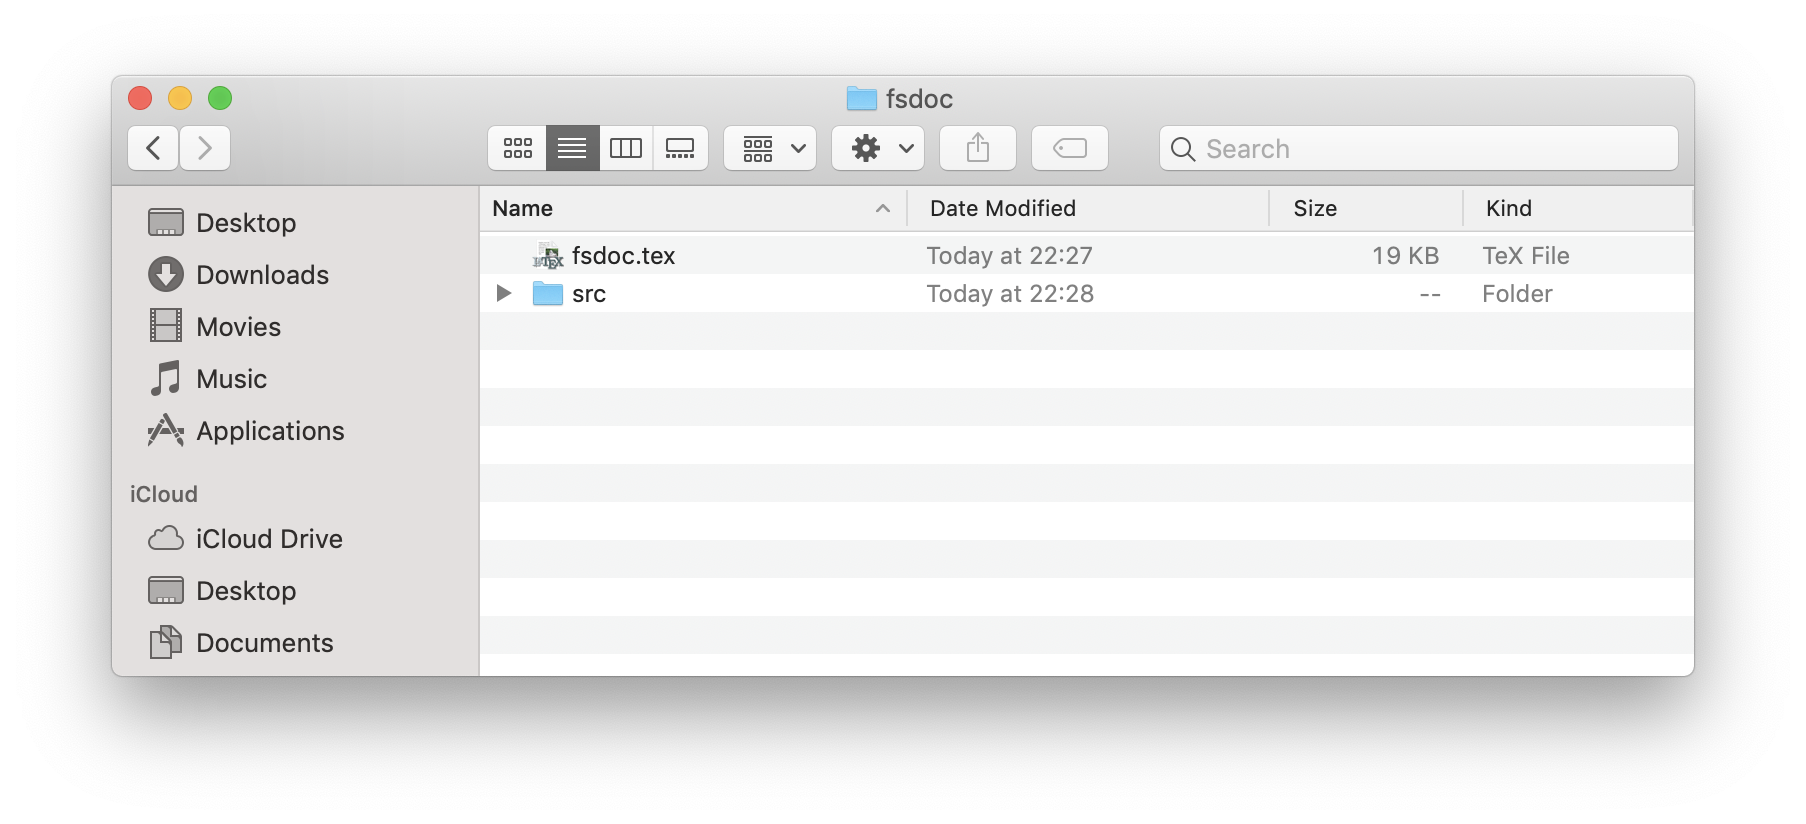
\includegraphics[width=12cm]{img/hidden}  
\end{figure}

\subsubsection{Arch}

The archived flag is not handled by the kernel itself. It can be set to mark that a file has been archived, such as during a backup operation.

\subsubsection{Schg}

\section{Extended Attributes}

Extended Attributes allow storing of arbitrary metadata of files on a file system. The concept of them was from the \gls{posix}\.1e draft which was withdrawn.

% https://unix.stackexchange.com/questions/489820/why-was-posix-1e-withdrawn

% https://git.kernel.org/pub/scm/linux/kernel/git/torvalds/linux.git/tree/include/uapi/linux/limits.h

The amount and size of attributes that can be set depend on the filesystem. Some filesystems, such as \gls{fat}, do not support them at all, while others like the \gls{ext} family of filesystems limit them.

POSIX Extended Attributes are divided into different namespaces. The \emph{user} namespace has no restrictions on what attributes can be set. 

\subsection{Capabilities}

\subsection{Access Control Lists}

\gls{acl} is a feature by which access to filesystem entries can be controlled more finely than with UNIX permissions\footnote{See \texttt{man acl} for more information}.


\section{Alternate File Streams}

\subsection{\gls{hfs+} Resource Fork}

A resource fork is a section of a file besides the file's actual contents that can be used to store structured data besides the unstructured data of the file itself. They appear as the extended attribute \verb|com.apple.ResourceFork|. 

Apple has a special syntax that can be used to access these forks with the standard \gls{posix} \gls{api} and tools. Given a file \verb|filename|, the special path \verb|filename/..namedforks/rsrc| can be used to access the resource fork.

\begin{verbatim}
$ touch file
$ echo hi > file/..namedforks/rsrc
$ cat file
$ cat file/..namedforks/rsrc
hi  
\end{verbatim}

Using \verb|ls -l@|, the extended attributes of the file can be listed, revealing the resource fork attribute.

\begin{verbatim}
$ ls -l@ file
-rw-r--r--@ 1 pelsen  staff  0 Sep 27 22:49 file
        com.apple.ResourceFork  3  
\end{verbatim}

These resource forks are a feature carried over from classic MacOS, and are not really used anymore. In fact, the \gls{api} to access them, \emph{Resource Manager}, have been removed. There are, to the best of my knowledge, no other named forks apart from the resource fork exposed.

\subsection{\gls{ntfs} Alternate Data Streams}

% https://www.borncity.com/blog/2018/09/22/infos-zu-windows-ntfs-alternative-data-streams/

\gls{ntfs} supports alternate data streams, which are used by Microsoft to tag downloaded files as being unsafe. It is also an interesting way to hide malware.

\section{Virtual Filesystems}

\subsection{Proc}

\subsection{Sys}


\printglossaries





\end{document}